\documentclass{book}
\usepackage{../notes}
\linespread{1.1}

\begin{document}
    \begin{titlepage}
        \centering
        \vspace*{\baselineskip}\vspace{200pt}
        \rule{\textwidth}{1.6pt}\vspace*{-\baselineskip}\vspace*{2pt}
        \rule{\textwidth}{0.4pt}\\[\baselineskip]
        {\Huge \bfseries \MakeUppercase{Physics 105} NOTES}\\[0.2\baselineskip]
        \rule{\textwidth}{0.4pt}\vspace*{-\baselineskip}\vspace{3.2pt}
        \rule{\textwidth}{1.6pt}\\[\baselineskip]
        \scshape
        Typeset notes for Physics 105: Analytic Mechanics\\
        \par
        \vspace*{2pt}
        {\Large Andrew Binder and Eric Du}\\
        {\large University of California, Berkeley\par}
        {\scshape Spring 2023} \\
    \end{titlepage}
    \setcounter{chapter}{-1}


    \chapter{Introduction}

    \begin{itemize}
        \item Instructor: Prof. Dan McKinsey
        \item Office Hours: Tuesdays, 2:30pm in 441 Physics South
        \item Grading:
        \begin{itemize}
            \item 30\% Homework
            \item 20\% Midterm 1
            \item 20\% Midterm 2
            \item 30\% Final
        \end{itemize}

        The grade bins for this class are fixed, and they will not be altered throughout the semester.
    \end{itemize}

    The first lecture of Physics 137A was held on  \textbf{Wednesday, August 24}. It covered the basics of the course syllabus and an introduction of blackbody radiation.

      \section{Why Quantum Mechanics?}
        Quantum mechanics was developed as a way to better describe physical observations. By the eighteenth century, we effectively mastered principles of Newtonian mecahnics, but we could not describe what was happening when objects glow when heated. So before we begin studying quantum mechanics, let's take a look at how we got here.

      \section{Blackbody Radiation}
        Blackbody radiation refers to the phenomenon that when a solid object, such as a cube of matter, is heated to a temperature $T$, it begins to glow.

        \begin{itemize}
          \item \textbf{1742:} It was observed that different objects (made from different materials) at the same temperature glow the same colour.
          \item \textbf{1800s:} The methods of spectroscopy get better, and we are now able to analyze light to a much higher degree of precision.
          \item \textbf{1854:} Kirchoff develops the modern theory of blackbody radiation. He imagined that there is a function $R(\lambda, T)$ which represents the emissive power per unit area of a blackbody. He also developed a the modern model of a blackbody $-$ an object that allows light and bounces many times, and it generates a temperature $T$ due to the bouncing. Here's an example of $R(\lambda, T)$ vs. $\lambda$:

          \begin{center}
            \begin{tikzpicture}
              \begin{axis}
                \addplot[color=red]{1e8* x/(e^x - 1)};
              \end{axis}
            \end{tikzpicture}
          \end{center}
        \end{itemize}

        There are a few characteristics of this curve that make intuitive sense. At $\lambda = 0$, there is no wave, so the blackbody radiation intensity should be 0. At large wavelengths, the light carries very low energy, and thus the radiation intensity is also very low.

        As this curve represents emissive power per unit area, the area (the integral) under the curve is finite, and describes the total emissive power. Stefan's law then states that the total radiation is proportional to $T^4$. Mathematically speaking, this means that

        \[ R(T) = \int_0^\infty R(T, \lambda) d\lambda = \sigma T^4\]

        Wein's law describes a relationship between the maximum wavelength of a blackbody curve to its temperature. Specifically, he found that $\lambda_{max}T = 2.898 \times 10^{-3}$, or in other words $\lambda_1 T_1 = \lambda_2T_2$.

        Then, Rayleigh and James calculated, numerically, that at high wavelengths this curve is approximated by

        \begin{equation}\label{classical blackbody equation}
        R(T) = \frac{8\pi k_B T}{\lambda^4}
        \end{equation}

        Notice that we have $\lambda^4$ in the denominator of this equation, meaning that our function should, in theory asymptote very quickly at low $\lambda$ values, However, this is not what we see in experiments! This discrepancy between the classical theory and observed is most commonly referred to as the \textbf{ultraviolet catastrophe.}

      \section{Derivation from First Principles}

      Let's now go back to first principles and try to build up a black body and see how it behaves. For simplicity, consider a cube of side length $L$ [INSERT TIKZ HERE]. Now, recall standing waves on a line: [INSERT TIKZ HERE] To figure out the eigennodes for such a setup, all we do is solve the wave equation we learned in E\&M:
      $$\nabla^2\psi(\vec{r},t) = \frac{1}{c^2}\frac{\partial^2}{\partial t^2}\psi(\vec{r},t)$$
      The quantum version of this equation will look similar, so it's good to remind ourselves of it. This is a second-order differential equation, which means that we need to specify the boundary conditions. In this case, our boundary condition is that $\psi$ must vanish at the cavity walls:

      $$\psi(x=0,y,z,t) = \psi(x=L,y,z,t) = 0$$
      From this, we get our standard solution of a sine wave:
      $$\psi(\vec{r},t) = A(t)\sin(k_xx)\sin(k_yy)\sin(k_zz)$$
      Here, $k_i = \frac{n_i\pi}{L}$. In other words, our equation is of the form $A(t)B(x,y,z)$. Essentially, we've separated the time parts and the space parts into different pieces, which is exactly what we would expect in the standing wave case. Mixing them together gives us traveling waves. If we now consider an electron in our box, we get an oscillating EM field, which will be important when we continue this next lecture.

    \chapter{Lecture 2 (01/19)}

This lecture was held on \textbf{January 19th, 2023}. It covered the equations of motion for damped and driven oscillators, as well as their applications in modern circuits.

\section{Last time: The Free Oscillator}

On Tuesday we explored oscillatory mechanics where there were no other forces besides the restoring force. However, in most systems, we will always have some kind of \textit{daming force} which impedes motion. This doesn't always have to be the case, but we will first explore a damping force which is proportional to the velocity: 

\[ \vec f = b \vec v\]

Under this, we now have the restoring force and the damping force, so Newton's second law now reads: 

\[ m \ddot x + b \dot x + kx = 0\] 

And so if we let $\beta = \frac{b}{2m}$ (we'll see later why this substitution is useful), then we can write

\[ \ddot x + 2\beta x + \omega_0^2 x = 0\]

The nature of these differential equations is that due to their linearity, if we find two independent solutions $x_1(t)$ and $x_2(t)$, then in general their solution will be a linear combination of the two: 

\[ x(t) = C_1x_1(t) + C_2x_2(t)\] 

We saw that exponentials worked before, let's have that as our main guess. Let 

\[ x(t) = e^{rt} \implies \dot x(t) = re^{rt}, \ddot x(t) = r^2e^{rt}\] 

Plugging this in, we get: 

\begin{align*}
    r^2e^{rt} + 2\beta r e^{rt} + \omega_0^2e^{rt} &= 0\\
    \therefore r^2 + 2\beta r + \omega_0^2 &= 0
\end{align*}

This is quadratic in $r$, so therefore we have solutions $r = -\beta \pm \sqrt{\beta^2 - \omega_0^2}$. Now, we can then write

\begin{align*}
    r_1 &= -\beta + \sqrt{\beta^2 - \omega_0^2}\\
    r_2 &= -\beta - \sqrt{\beta^2 - \omega_0^2}
\end{align*}

so the general solution now becomes: 

\[ x(t) = C_1e^{r_1t} + C_2e^{r_2t} = e^{-\beta t} \left( C_1e^{\sqrt{\beta^2 - \omega_0^2} t } + C_2e^{-\sqrt{\beta^2 - \omega_0^2}t}\right)\]

This equation makes sense intuitively, since a large value of $\beta$ generates a faster decay, which makes sense since $\beta$ refers to the damping constant. 

Now we have 3 cases that we want to analyze: 

\begin{enumerate}[label = (\alph*)]
    \item Underdamped: $\omega_0^2 > \beta^2$ 
    \item Critical damping: $\omega_0^2 = \beta^2$
    \item Overdamped: $\omega_0^2 < \beta^2$
\end{enumerate}

As it will turn out, only the overdamping will give us oscillatory motion.

\subsection{Case 1: Underdamped Oscillation} 

Here we look at the case where $\omega_0^2 > \beta^2$. If this is the case, then we can write $\sqrt{\beta^2 - \omega_0^2} = i\sqrt{\omega_0^2 - \beta^2} = i\omega_1$, with $\omega_1 = \sqrt{\omega_0^2 - \beta^2}$

\begin{insight*}{}{}
    if $\beta = 0$, then we exactly recover the solution that we got last time: 

    \[ x(t) = C_1e^{\sqrt{-\omega_0^2}t} + C_2e^{-\sqrt{-\omega_0^2}t} = C_1e^{i\omega_0t} + C_2e^{-i\omega_0t}\]

    This is a good way to check that what we're doing still makes sense.
\end{insight*}

There's also the case where we get \textit{weak underdamping}, where essentially we have $\beta \ll \omega_0$, so we get instead $x(t) = e^{-\beta t}\left(C_1e^{i\omega_1t} + C_2e^{-i\omega_1t}\right)$. Here, the $e^{-\beta t}$ term goes to zero over time, and the second term is just oscillation with $\omega_0 \to \omega_1$, so we can interpret this as an oscillation with an envelope of a decaying exponential. A diagram representation: 

\begin{center}
    \begin{tikzpicture}[samples=100, domain=0:5]

        \draw[->] (0, 0) -- (5.5,0) node[right] {$t$};
        \draw[->] (0,-2) -- (0,2) node[above] {$x(t)$};

        \draw[color=blue] plot (\x, {cos(5 * \x r) *exp(-0.5 * \x)}) node[above] {$x(t)$};
        \draw[color=red, dashed] plot (\x, {exp(-0.5 * \x)});
        \draw[color=red, dashed] plot (\x, {-exp(-0.5 * \x)});
        \node[color=red] at (3, 0.7) {$e^{-\beta t}$};
        \node[color=red] at (3, -0.7) {$-e^{-\beta t}$};
    \end{tikzpicture}
\end{center}

Here, the red dashed lines represent the envelope, and the $x(t)$ represents the actual motion. As we can see, the oscillation goes to zero over time, which makes sense since the damping force is constantly taking away energy. 

\subsection{Case 2: Damped Oscillation}

Now we look at $\omega_0^2 < \beta^2$. Here, the exponentials are real, so we can write:

\[ x(t) = C_1e^{-(\beta - \sqrt{\beta^2 - \omega_0^2})t} + C_2 e^{-(\beta + \sqrt{\beta^2 - \omega_0^2})t}\] 

On large time scales, we can see that the oscillation is dominated by the slower of the two exponentials (the faster one just dies out quicker, so we don't see it for large times). Interestingly, the rate of decay is lower if $\beta$ is larger, and we can see that since the exponentials get larger. 

When solving these problems, there are three cases we need to specifically look at if we let $x(0) = x_0 > 0$: 

\begin{itemize}
    \item $\dot{x_0} > 0$ such that we reach the maximum then the pendulum comes back.
    \item $\dot{x_0} < 0$ but we approach $x = 0$ but we do not go past. 
    \item Same as the previous case, but we do end up going past $x = 0$.
\end{itemize}

\subsection{Case 3: Critical Damping}

Now we look at $\omega_0^2 = \beta^2$, the most interesting case. Here, this means that the roots of $r^2 + 2\beta r + \omega_0^2 = 0$ are equal, so our solution becomes

\[ x(t) = e^{\beta t}\] 

Well we know that this differential equation has two solutions, and there is indeed a second solution, $x(t) = xe^{\beta t}$. We can check that it satisfies the differential equation by plugging it in (you can do this on your own time)

A critically damped oscillator will approach equilibrium the fastest. This has important design consequences $-$ in times where we want to reduce oscillation, critically damped systems are especially useful. Below is an illustration of this: 

\begin{center}
    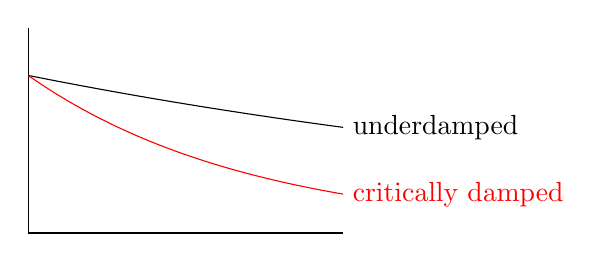
\begin{tikzpicture}[domain=0:2, samples=50, scale=2]
        \draw(0, 0) -- (2, 0);
        \draw(0, 0) -- (0, 1.3);
        \draw[color=black] plot (\x, {exp(-0.2* \x)}) node[right] {underdamped};
        \draw[color=red] plot (\x, {exp(-0.7 * \x)}) node[right] {critically damped};
    \end{tikzpicture}
\end{center}

Both of these curves are exponential decay curves, but the critically damped one goes to zero much faster than any other damping.

\section{Driving Forces}

Now imagine instead of a resistive force, that we have a driven force instead. That is, our equation of motion now looks like this: 

\[ F = -kx - bx + F_0 \cos(\omega t)\] 

where $F_0 \cos(\omega t)$ denotes the driving force, with $\omega$ being the angular frequency of the driving force. Therefore, we have the differential equation:

\[ \ddot x + 2\beta x + \omega_0^2x = f_0 \cos(\omega t)\] 

where $f_0 = \frac{F_0}{m}$, and $\beta$ is defin in the same way as before. This differential equation has two solutions: 

\begin{itemize}
    \item A homogeneous solution $x_h(t)$, which solves the differential equation when the right hand side is 0. 
    \item A particular soluiton, $x_p(t)$, which solves the differential equation while replicating the right hand side. 
\end{itemize}

Then, if we can find these two solutions, then we can combine them together: 

\[ x(t) = x_h(t) + x_p(t)\] 

We already know $x_h(t)$ from the earlier section, so if we can find an $x_p(t)$, then we have the full solution to the problem. We've seen before that sines and cosines seem to work well with oscillations, so why not try the solution $x_p(t) = A\cos(\omega t - \delta)$. Plugging this in, we get: 

\begin{align*}
    -A\omega^2 \cos(\omega t - \delta) - 2\beta A \omega \sin (\omega t - \delta) + \omega_0^2 A \cos(\omega t - \delta) = f_0 \cos \omega t\\
    f_0 \cos (\omega t) - A(\omega_0^2 - \omega^2)\cos(\omega t - \delta) + 2\beta A \cos(\omega t - \delta) = 0
\end{align*}

Now we use the trigonometric identities:

\begin{align*}
    \cos(\alpha - \beta) &= \cos \alpha \cos \beta + \sin \alpha \sin \beta\\
    \sin(\alpha - \beta) &= \sin \alpha \cos \beta - \cos \alpha \sin \beta
\end{align*}
    
Doing so we get the equation:


\[ \left \{ f_0 - A\left[ (\omega_0^2 - \omega^2)\cos \delta + 2\omega \beta \sin \delta \right]\right \} \cos (\omega t) -  \left \{A\left[ (\omega_0^2 - \omega^2)\sin \delta - 2\omega \beta \cos(\omega t)\right] \right \} \sin(\omega t) = 0\] 

Since $\sin(\omega t)$ and $\cos(\omega t)$ are linearly independent functions, this euqation is only satisfied when both terms are zero. From the first term, we get:

\begin{align*}
    \tan \delta &= \frac{2\omega \beta}{\omega_0^2 - \omega^2} \\
    \therefore \delta &= \tan^{-1}\left(\frac{2\omega \beta}{\omega_0^2 - \omega^2}\right)
\end{align*}

Therefore, 

\[ \sin \delta = \frac{2\omega \beta}{\sqrt{(\omega_0^2 - \omega^2)^2 + 4\omega^2 \beta^2}} \phantom{aaa} \cos \delta = \frac{\omega_0^2 - \omega^2}{\sqrt{(\omega_0^2 - \omega^2)^2 + 4\omega^2 \beta^2}}\]

From the cosine term, we get: 

\begin{align*}
    A &= \frac{f_0}{(\omega_0^2 - \omega^2)\cos \delta + 2\omega \beta \sin \delta}\\
    &= \frac{f_0}{\sqrt{(\omega_0^2 - \omega^2) + 4\omega^2 \beta^2}}
\end{align*}

so now we finally have the particular solution: 

\[ x_p(t) = A\cos(\omega t - \delta) = \frac{f_0 \cos (\omega t - \delta)}{\sqrt{(\omega_0^2 - \omega^2) + 4\omega^2 \beta^2}}\]

So our general solution, (again $x(t) = x_h(t) + x_p(t)$) is

\[ x(t) = C_1e^{r_1t} + C_2e^{r_2t} + A\cos(\omega t - \delta)\] 

Note that for large time, the $x_h(t)$ terms die out, but the $x_p(t)$ terms don't, and dominate for large time $t \gg \frac 1 \beta$. In other words: 

\[ x(t \gg \frac{1}{\beta}) = x_p(t)\] 

\subsection{The phase difference}

Earlier we said that $\delta$ represents the phase differene between the action and the resulting motion: 

\[ \delta = \tan^{-1}\left(\frac{2\omega \beta}{\omega_0^2 - \omega^2}\right)\] 

For a fixed $\omega_0$, as $\omega$ increases from 0, we get that the phase increases from $\delta = 0$ to $\delta = \pi/2$ at $\omega = \omega_0$ and $\delta \to \pi$ as $\omega \to \infty$.

\subsection{Amplitude} 

At large times, it's useful to look at the effect of $\omega$ on the amplitude by looking at $x_p(t)$. To find where $A$ is maximized, we simply take $\frac{dA}{d\omega} = 0$, giving us $\omega_2 = \sqrt{\omega_0^2 - 2\beta^2}$, so the resonance frequency is lowered as damping $\beta$ is increased. This makes sense intuitively, since the larger value of $\beta$ means that our oscillation decays much faster. 

\begin{insight*}{}{}
    Note that we don't get any resonance frequencies for $\beta^2 > \omega_0^2/2$, since that's when the square root becomes complex-valued.
\end{insight*}

[INSERT TIKZ HERE]

\section{Summary} 

In summary, so far we've looked at free, damped and driven oscillations: 
\begin{itemize}
    \item Free oscillations: $\omega_0 = \frac{k}{m}$
    \item Damped oscillations: $\omega_1 = \omega_0^2 - \beta^2$
    \item Driven oscillations: $\omega_2 = \omega_0 - 2\beta^2$
\end{itemize}

This set of relations gives us $\omega_0 > \omega_1 > \omega_2$. The maximum amplitude is given by 

\[ A_{max} = \frac{f_0}{\sqrt{4\omega^2\beta^2}} = \frac{f_0}{2\omega \beta}\]

This equation tells us that if we make $\beta$ smaller, then $A_{max}$ increases and also becomes taller and narrower. We define the \textit{full width half maximum} ($\text{FWHM} = 2\beta$ ) to quanitfy this value. 

\subsection{Aside: Quality Factor} 

We sometimes define a quality factor $Q$ as the ration of the resonance position $\omega_0$ to its width $2\beta$:

\[ Q = \frac{\omega_0}{2\beta}\] 

This means that large values of $Q$ correspond to narrow resonance, and small values correspond to a wide resonance. 

\section{Application: LC Circuits}

We've learned in electricity and magnetism (and also 5BL) that a simple LC circuit also behaves like an oscillator, since it follows the equation: 

\[ L \frac{dI}{dt} + \frac 1c \int I \ dt = 0\] 

or in terms of the charge $q$: 

\[ L \ddot q + \frac{1}{c} q = 0\] 

The solutions are of the same form since the only thing we've changed here are the variable names: $q(t) = q_0 \cos(\omega t)$. Overall, we can just perform the substtution of letters: 

\[ m \to L \phantom{aa} x \to q \phantom{aa} \frac 1k \to c \phantom{aa} \dot x \to I\] 

Similarly, adding a resistance will give us the equivalent of a damping term, and adding an AC power generator is the same as adding a driving force to the system. Again, the nature of these system is the exact same as what we just solved for, so the equations of motion remain the same as well.




 
	\chapter{Lecture 9}

Lecture 9 was held on [INSERT DATE HERE], and it covered [INSERT TOPIC HERE]

\section{Orbital Motion Revisited}
Let's look back at our expression for the path of a particle $\phi(r)$:
\[ \phi(r) = \int \frac{\frac{\ell}{r^2} dr}{\sqrt{2\mu\left( E - U - \frac{\ell^2}{2\mu r^2} \right) } }\]
If we assume that we're talking about the gravitational force here, the we can write $U = -\frac{Gm_1m_2}{r} 
\equiv - \frac{\gamma}{r}$. And so we instead just have to solve the integral:
\[ \phi(r) = \int \frac{\frac{\ell}{r^2} dr}{\sqrt{2\mu\left( E + 
\frac{\gamma}{r}-\frac{\ell^2}{2\mu r^2} \right) } }\]
To make this integral easier, we perform a u-substitution of $u = \frac{1}{r}$ and $du = -\frac{1}{r^2}$ so we 
have:
\[ \phi(r) = -\int \frac{du}{\sqrt{\frac{2 \mu E}{\ell^2} + \frac{2 \mu \gamma}{\ell^2}u - u^2} }\]
The solution to this integral can be calculated using an integral table: 
\[ \int \frac{dx}{\sqrt{ax^2 + bx + c} } = -\frac{1}{\sqrt{-a} }\sin^{-1}
\left[ \frac{2ax+b}{\sqrt{b^2 - 4ac} }\right] + C\]
\begin{insight*}{}
		Here, it's important to note that since $a = -1$ in our original equation, so that the fraction
		$\frac{1}{-\sqrt{a} }$ is a real quantity. Since we need to enforce that $\phi(r)$ must also be real 
		then we also require that $2ax + b < \sqrt{b^2 - 4ac}$, otherwise the $\sin^{-1}$ term would also return
		a complex value.
\end{insight*}

Using this solution, we then have: 
\[ \phi + C = \sin^{-1}\left[\frac{-\frac{2}{r} + 
\frac{2\mu \gamma}{\ell^2}}{\sqrt{\left[\frac{2\mu\gamma}{\ell^2}\right]^2+ 8 \frac{\mu E}{\ell^2}}}\right]\] 
Taking the sine now, we can get: 
\[ \sin(\phi + C) = \frac{-\frac{2}{r} + 
\frac{2\mu \gamma}{\ell^2}}{\sqrt{\left[\frac{2\mu\gamma}{\ell^2}\right]^2 + 8 \frac{\mu E}{\ell^2}} }\]
Then we can cancel the constant by allowing our $\phi$ to start at a moment where $C = \frac{\pi}{2}$, and so we
get instead: 
\[ \cos \phi = \frac{\frac{\ell^2}{\mu \gamma}\frac{1}{r}-1}{1 + \frac{2E\ell^2}{\mu \gamma^2}}\]
Here, we can define the constants: 
\[ c \equiv \frac{\ell^2}{\gamma \mu} \ \ \ \ \epsilon \equiv \sqrt{1 + \frac{2E\ell^2}{\mu \gamma^2}} \]
so we get the simple looking equation: %include a colorbox here
\begin{theorem*}{}
		For two particles moving in orbit with one another under a force that varies with $\frac{1}{r^2}$, the 
		orbit of one particle in terms of the center of mass frame is:

		\[ r(\phi) = \frac{c}{1+\epsilon \cos \phi}\]
		
\end{theorem*}
This gives us an equation for $r$ in terms of the angle $\phi$, which is measured as the angle between the x axis
and the line connecting the focus to the orbiting body. This equation also happens to be the equation of a conic
section with one focus at the origin, directly implying that planetary motion always traces out conic sections. 
\begin{insight*}{}
		There is nothing really special about the gravitational force either -- any central force that varies like
		$\frac{1}{r^2}$ will naturally give us these orbit equations, since we didn't really assume anything 
		besides substituting $U = -\frac{\gamma}{r}$.
\end{insight*}
\section{Alternate Method} 
Alternatively, we could have also determined $r(\phi)$ by analyzing forces, by using the equation:
\[ \dv[2]{u}{\phi} + u = -\frac{u}{\ell^2}\frac{1}{u^2}F(u)\] 
If we assume that $F$ follows an inverse-square relation, then we ge;
\[ F(r) = -\gamma u^2\]
(here $\gamma$ eats up all the constants), and so we get the differential equation: 
\[ u''(\phi) = -u(\phi) + \frac{\gamma \mu}{\ell^2}\]
Note that here, we have a differential equation that almost looks like simple harmonic motion, but we have a 
constant term now. To get rid of this, we introduce the substitution
\[ w(\phi) = u(\phi) - \frac{\gamma \mu}{\ell^2}\]
so we get:
\[ w''(\phi) = -w(\phi)\] 
which has a solution: 
\[ w(\phi) = A \cos(\phi - \delta)\]
We can then cancel $\delta$ with ah appropriate choice for $\phi = 0$, so therefore our general solution $u(\phi)$
is:
\[ u(\phi) = \frac{\gamma \mu}{\ell^2} + A \cos \phi = \frac{\gamma \mu}{\ell^2}(1 + \epsilon \cos \phi)\]
So finally: 
\[ r(\phi) = \frac{c}{1 + \epsilon \cos \phi}\]
which is the same equation we've recovered before. This derivation using forces and solving the differential 
equation is what Taylor goes through, but either method is obviously valid. To find $\epsilon$, we can also notice
that $E = U_{eff}(r_{min})$ to derive an expression for $\epsilon$ in terms of the constants we had before. The 
expression for $E$ then becomes: 
\[ E = U(r_{min}) + \frac{\ell^2}{2 \mu r_{min}^2} = \frac{1}{2r_{min}}\left( \frac{\ell^2}{\mu r_{min}} 
- 2\gamma \right) \]
We also know that $r = r_{min}$ when $\cos \phi = 1$, so therefore $r_{min} = \frac{c}{1 + \epsilon}$. Plugging
this in, we get:
\begin{align*}
		E &= \frac{1}{2\left( \frac{c}{1 + \epsilon} \right) }\left( \frac{\ell^2}{\mu\left( \frac{c}{1 +
			\epsilon} \right) }- 2 \gamma\right)\\
			&= \frac{1}{2\left( \frac{\ell^2/\gamma \mu}{1 +
			\epsilon}\right)}\left( \frac{\ell^2}{\mu\left( \frac{\ell^2/ \gamma \mu}{1 +
			\epsilon}\right) } - 2 \gamma \right) \\
			&= \frac{\gamma \mu (1 + \epsilon)}{2\ell^2}[\gamma(1 + \epsilon) - 2 \gamma] \\
			&= \frac{\gamma^2\mu}{2\ell^2}(\epsilon^2 - 1)
\end{align*}
So this then gives us the relation that we're looking for:
\[ \epsilon = \sqrt{1 + \frac{2E\ell^2}{\mu \gamma^2}} \]
\begin{notation*}{Eccentricity}
		The quantity $\epsilon$ is also called the \textit{eccentricity} of orbit, and roughly translates to how
		``squashed" the orbit looks.
\end{notation*}
This equation actually has very profound consequences. For one, it tells us that if $E < 0$ then we have $\epsilon
< 1$, so this corresponds to bound orbits. Otherwise, if $E > 0$, then this corresponds instead to unbound 
orbits.
\begin{insight*}{}
		This result also matches our previous intuition about bounded orbits. Recall the potential energy curve:

		\begin{center}
				\begin{tikzpicture}[yscale=0.3, xscale = 0.9]
                    \draw[domain=0.34:10, samples=500, color=red] plot (\x, {-6/\x + 3/(\x^2)});
                    \draw[very thick, -stealth] (0, 0) -- (11, 0) node[right] {$r$};
                    \draw[very thick, -stealth](0, -5) -- (0, 10) node[above]{$V(r)$};
					\draw[dashed, blue] (11, 3) node[right] {$E > 0$} -- (0, 3);
					\draw[dashed, blue] (11, -1) node[right] {$E < 0$} -- (0, -1);
					\draw[dashed] (5.4495, -4) node[below] {$r_{max}$} -- (5.4495, -1) -- (5.4495, 0);
					\draw[dashed] (0.550, -4) node[below] {$r_{min}$} -- (0.550, -1) -- (0.550, 0);
                \end{tikzpicture}
            \end{center}
		Notice that for $E < 0$, then our energy intersects our curve at 2 locations, giving us
		an $r_{min}$ and $r_{max}$ matching the fact that the orbit is bounded. But, for $E > 0$, notice that we
		only have one intersection $r_{min}$, matching the fact that the orbit is unbounded. 
\end{insight*}
Looking back at our equation $r(\phi)$, 
\[ r(\phi) = \frac{c}{1 + \epsilon \cos \phi}\] 
notice that if $\epsilon < 1$, then the denominator in this expression never vanishes, so $r(\phi)$ is bounded for
all $\phi$. On the other hand, if $\epsilon \ge 1$, then the denominator vanishes for some angle and $r(\phi)$ 
approaches infinity as $\phi$ approaches that angle, corresponding to an unbounded orbit.
\section{Bounded Orbits}
Let's now consider the case where $\epsilon < 1$. Then, our denominator oscillates between: 
\[ r_{min} = \frac{c}{1 + \epsilon} \ \ \text{and} \ \ r_{max} = \frac{c}{1 - \epsilon}\] 
Since this is a bounded orbit, then $r(\phi)$ clearly must be periodic with a period of $2\pi$, and the orbit 
should close on itself after one revolution. If we then perform a change of variables and write $r = \sqrt{x^2 + 
y^2} $ and $\cos \phi = x/r$, then we get:
\begin{align*}
		r &= \frac{c}{1 + \epsilon cos \phi} \\
		r\left( 1 + \frac{\epsilon x}{r} \right) &=  c \\
		\therefore r &=  c - \epsilon x \\
\end{align*}
And so now completing the square and setting $r^2 = x^2 + y^2$: 
\begin{align*}
		r^2 = (c - \epsilon x)^2 &=  x^2 + y^2 \\
		c^2+ \epsilon^2 x^2 -2c\epsilon x &=  x^2 + y^2 \\
		(1 - \epsilon^2) x^2 + 2c\epsilon x + y^2 &=  c^2 \\
		(x + d)^2 + \frac{y^2}{1 - \epsilon^2} &= \frac{c^2}{(1 - \epsilon^2)} + d^2\\
		(x + d)^2 + \frac{y^2}{1 - \epsilon^2} &=  \frac{c^2}{(1 - \epsilon^2)} +
		\frac{c^2\epsilon^2}{(1 - \epsilon^2)^2} \\
		(x + d)^2 + \frac{y^2}{1 - \epsilon^2} &=  \frac{c^2 - c^2 \epsilon^2 + c^2 \epsilon^2}{(1 -
		\epsilon^2)^2} \\
		(x + d)^2 + \frac{y^2}{1 - \epsilon^2} &=  \frac{c^2}{1 - \epsilon^2} \\
		\frac{(x+d)^2}{a^2} + \frac{y^2}{b^2} &= 1
\end{align*}
This is the equation for an ellipse, with $a = \frac{c}{1 - \epsilon^2}$, $b = \frac{c}{\sqrt{1 - \epsilon^2} }$ 
and $d = \frac{c \epsilon}{1 - \epsilon^2} = a\epsilon$. The center of the ellipse is offset from the origin by 
$d$ along the $x$-axis, and the ratio of major and minor axes is: 
\[ \frac{b}{a}= \sqrt{1 - \epsilon^2} \]
This leads us to Kepler's first law: 
\begin{theorem*}{}
	Planets and bound comets follow orbits that are ellipses with the sun at one focus.	
\end{theorem*}
Further, plugging in $c = \frac{\ell^2}{\gamma \mu}$ and $\epsilon = \sqrt{1 + \frac{2 E \ell^2}{\mu \gamma^2}}$
then we can also see that: 
\begin{align*}
		a &= \frac{c}{1 - \epsilon^2} = \frac{\gamma}{2|E|}\\
		b &=  \frac{c}{\sqrt{1 - \epsilon^2} } = \frac{\ell}{2\mu |E|} \\
\end{align*}
And so we can see that the major axis $2a$ depends only on the energy, while the minor axis depends on both the 
energy and the momentum.



\end{document}
